\documentclass[nobib]{tufte-handout}

\title{Föreläsning 2: Kombinatoriska bevis, binomialsatsen $\cdot$ 1MA020}

\author[Vilhelm Agdur]{Vilhelm Agdur\thanks{\href{mailto:vilhelm.agdur@math.uu.se}{\nolinkurl{vilhelm.agdur@math.uu.se}}}}

%\date{15 januari 2023}


%\geometry{showframe} % display margins for debugging page layout

\usepackage{graphicx} % allow embedded images
  \setkeys{Gin}{width=\linewidth,totalheight=\textheight,keepaspectratio}
  \graphicspath{{graphics/}} % set of paths to search for images
\usepackage{amsmath}  % extended mathematics
\usepackage{booktabs} % book-quality tables
\usepackage{units}    % non-stacked fractions and better unit spacing
\usepackage{multicol} % multiple column layout facilities
\usepackage{lipsum}   % filler text
\usepackage{fancyvrb} % extended verbatim environments
  \fvset{fontsize=\normalsize}% default font size for fancy-verbatim environments

\usepackage{color,soul} % Highlights for text

% Standardize command font styles and environments
\newcommand{\doccmd}[1]{\texttt{\textbackslash#1}}% command name -- adds backslash automatically
\newcommand{\docopt}[1]{\ensuremath{\langle}\textrm{\textit{#1}}\ensuremath{\rangle}}% optional command argument
\newcommand{\docarg}[1]{\textrm{\textit{#1}}}% (required) command argument
\newcommand{\docenv}[1]{\textsf{#1}}% environment name
\newcommand{\docpkg}[1]{\texttt{#1}}% package name
\newcommand{\doccls}[1]{\texttt{#1}}% document class name
\newcommand{\docclsopt}[1]{\texttt{#1}}% document class option name
\newenvironment{docspec}{\begin{quote}\noindent}{\end{quote}}% command specification environment

\include{mathcommands.extratex}

\begin{document}

\maketitle% this prints the handout title, author, and date

\begin{abstract}
\noindent
Vi fortsätter på förra föreläsningens idéer om kombinatoriska bevis och att räkna saker på två olika sätt. Sedan tillämpar vi detta på att bevisa binomialsatsen.
\end{abstract}

\section{Kombinatoriska bevis}

I slutet av förra föreläsningen diskuterade vi kombinatoriska bevis, och bevisade saker genom att räkna samma sak på två olika sätt. I denna föreläsningen fortsätter vi på det spåret, med fler bevis där vi hittar smarta sätt att räkna något.

\begin{example}\label{example_triangular_numbers}
  För $n\geq 0$, låt $S(n) = \sum_{k=1}^n k$. Vi vill bevisa att $S(n) = \frac{n(n+1)}{2}$.\sidenote[][-2cm]{Det sägs att den store matematikern Carl Friedrich Gauss en gång fick uppgiften att räkna ut $1+2+\ldots+100$ av en lat mellanstadielärare som ville hålla sina elever upptagna i en stund, och förbluffade sin lärare genom att hitta svaret på bara några sekunder och utan papper och penna.
  
  Han använde dock en annan metod än den vi använder, som inte involverade någon figur. Kan du komma på fler sätt att göra detta? (Eller Googla ``Gauss triangular numbers story'' om du bara vill veta svaret.)}

  Vi studerar ett rutnät av $(n+1)\times(n+1)$ punkter, såsom i figuren.

  \begin{figure}
    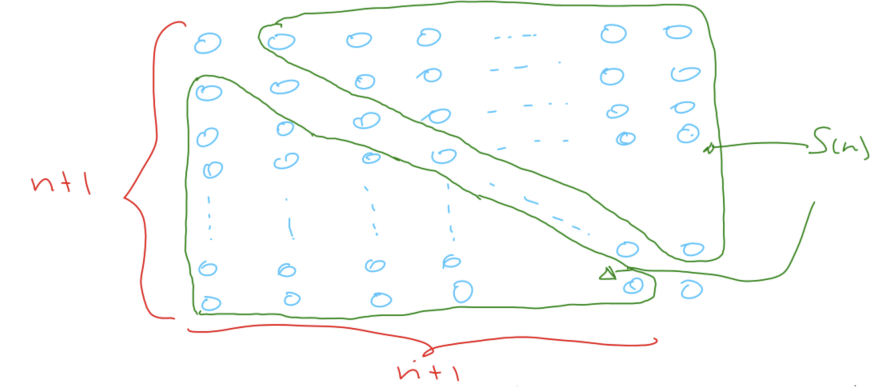
\includegraphics{graphics/counting_triangular_numbers_by_square.png}
    \caption[][2cm]{Ett rutnät av punkter. Figur tagen direkt från förra årets föreläsningsanteckningar.}
  \end{figure}
  
  Vi ser på den nedre gröna triangeln, och försöker räkna antalet punkter i den. Vi ser att den vänstra kolumnen har $(n+1)-1 = n$ punkter, den näst vänstraste har $(n+1)-2=n-1$ punkter, och så vidare till den näst längst till höger som har en punkt, och kolumnen längst till höger har noll punkter i den gröna triangeln.

  Alltså, om vi summerar över kolumnerna så får vi att det är totalt $n + (n-1) + \ldots + 2 + 1 = S(n)$ punkter i triangeln. Eftersom kvadraten så klart är helt symmetrisk är det lika många punkter i den övre gröna triangeln, och det är lätt att se att det är $n+1$ punkter på diagonalen.

  Alltså måste det totala antalet punkter i kvadraten vara $2S(n) + (n+1)$ -- men vi vet också, så klart, att det är $(n+1)^2$. Så om vi löser detta för $S(n)$ får vi att
    $$S(n) = \frac{(n+1)^2 - (n+1)}{2} = \frac{(n+1)((n+1)-1)}{2} = \frac{n(n+1)}{2}$$
  precis som vi önskade.
\end{example}

\begin{example}\label{example_counting_all_subsets}
  Bevisa att $\sum_{k=0}^n \binom{n}{k} = 2^n$.

  \begin{proof}
    Vi bevisar detta genom att bevisa att både vänster och höger led räknar antalet delmängder till en mängd av $n$ element, oavsett delmängdernas storlek.\sidenote[][]{Man kan också betrakta detta som att vi räknar antalet binära strängar av längd $n$ på två sätt, eftersom det finns en enkel bijektion mellan sådana och delmängder till en mängd $X$ av storlek $n$.
    
    Specifikt så fixerar vi en numrering av elementen av $X$, och säger att givet en binär sträng $x_1x_2\ldots x_n$ så får vi en delmängd $A\subseteq X$ genom att det första elementet av $X$ ligger i $A$ om $x_1=1$, det andra om $x_2=2$, och så vidare. På motsvarande sätt kan vi konstruera en binär sträng givet en delmängd.}

    För vänster led kan vi observera att antalet delmängder oavsett storlek är summan av antalet delmängder av varje given storlek. Vi vet sedan innan att en delmängd av storlek $k$ av en mängd av storlek $n$ kallas en kombination, och det finns $\binom{n}{k}$ stycken sådana. Alltså är det totala antalet delmängder $\sum_{k=0}^n \binom{n}{k}$, som önskat.

    För höger led använder vi multiplikationsregeln. För varje element i vår mängd har vi två val -- antingen tar vi med elementet, eller inte -- och vi har totalt $n$ stycken element för vilka vi behöver göra detta val. Så om vi multiplicerar antalet val vi har varje gång får vi $2\cdot2\cdot\ldots\cdot2 = 2^n$ stycken delmängder, som önskat.
  \end{proof}
\end{example}

\begin{proposition}[Pascals Identitet]
  För $1 \leq k \leq n$ gäller det att\sidenote[][]{Den här likheten säger exakt att Pascals triangel faktiskt innehåller binomialkoefficienterna.}
  
  \begin{marginfigure}
    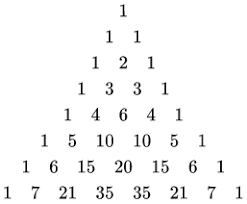
\includegraphics{graphics/pascals_triangle.png}
  \end{marginfigure}
  $$\binom{n}{k} = \binom{n-1}{k-1} + \binom{n-1}{k}.$$

  \begin{proof}[Algebraiskt bevis]
    \begin{align*}
      \binom{n-1}{k-1} + \binom{n-1}{k} &= \frac{(n-1)!}{(k-1)!((n-1)-(k-1))!} + \frac{(n-1)!}{k!((n-1)-k)!}\\
      &= (n-1)!\left(\frac{k}{k!(n-k)!} + \frac{(n-k)}{k!(n-k)!}\right)\\
      &= (n-1)!\frac{k + (n - k)}{k!(n-k)!}\\
      &= \frac{n!}{k!(n-k)!} = \binom{n}{k}.
    \end{align*}    
  \end{proof}

  \begin{proof}[Kombinatoriskt bevis]
    Låt $X$ vara en mängd av storlek $n$. Vi vet att $\binom{n}{k}$ räknar antalet delmängder av storlek $k$ till $X$. Låt oss komma på ett annat sätt att räkna antalet delmängder av storlek $k$, och se att det ger oss höger led.

    Välj ett godtyckligt element $x \in X$. För varje delmängd $A$ till $X$ så innehåller den antingen $x$, eller så gör den inte det. För att skapa oss en delmängd $A$ av storlek $k$ som innehåller $x$ lägger vi först in $x$ i $A$, och sedan lägger vi till ytterligare $k-1$ element från de återstående $n-1$ elementen. Antalet sätt att göra det vet vi är precis $\binom{n-1}{k-1}$

    Om vi i stället vill ha en delmängd $A$ som \emph{inte} innehåller $x$ så kan vi fritt välja $k$ element av de återstående $n-1$ elementen. Antalet sätt att göra det på vet vi är $\binom{n-1}{k}$.

    Så additionsprincipen säger oss att antalet sätt att välja en delmängd som innehåller $x$ eller inte innehåller $x$ -- vilket ju är alla delmängder -- måste vara summan, alltså $\binom{n-1}{k-1} + \binom{n-1}{k}$, såsom önskat.
  \end{proof}
\end{proposition}

\section{Binomialsatsen}

\begin{theorem}[Binomialsatsen]
  För varje heltal $n\geq 0$ gäller det att\sidenote[][]{Lägg märke till att vi inte är så precisa kring vad $x$ och $y$ är. I versionen ni lärde er i gymnasiet är de två reella tal, men egentligen är det här en likhet mellan polynom, som gäller mycket mer allmänt. Vi använder ju inte några specifika egenskaper hos de reella talen i det här beviset, bara räkneregler för polynom. När ni läser en kurs i algebra kommer ni se hur generellt den sortens räkningar fungerar.}
  $$(x + y)^n = \sum_{k=0}^n \binom{n}{k}x^{n-k}y^k$$
  \begin{proof}
    Studera uttrycket
    $$(x + y)^n = (x + y)(x + y)\ldots(x + y).$$

    Vad är det vi gör när vi expanderar ut detta uttrycket? Jo, vi väljer för varje parentes om vi tar ett $x$ eller ett $y$ -- eller uttryckt i kombinatoriska termer, vi bildar ett ord ur alfabetet $\{x, y\}$. Så för $n = 3$ får vi till exempel att
    $$(x+y)(x+y)(x+y) = xxx + xxy + xyy + yxx + yxy + yyy.$$

    Sedan kommer vi ihåg att multiplikation är kommutativt, så $xyy = yxy$. Alltså spelar det ingen roll i vilken ordning vi gjorde valen, bara hur många gånger vi valde $x$ och hur många gånger vi valde $y$.\sidenote[][]{Alltså, formulerat på ett annat sätt, etiketterna av ``när valdes vilken'' spelar ingen roll.}

    Så antalet gånger vi får en term som är lika med $x^{n-k}y^k$ kommer alltså vara antalet $\{x, y\}$-strängar med $k$ stycken $y$. Det antalet är så klart samma som antalet sätt att välja $k$ platser att skriva $y$ ur den totala mängden av $n$ platser -- det vill säga $\binom{n}{k}$.

    Vi har alltså sett att koefficienten framför $x^{n-k}y^k$ när vi förenklat uttrycket kommer att vara $\binom{n}{k}$. Eftersom detta argument fungerar för varje $k$ har vi bevisat satsen.
  \end{proof}
\end{theorem}

\section{Övningar}

\begin{xca}
  I Exempel \ref{example_triangular_numbers} såg vi att
  $$\sum_{k=1}^n k = \frac{n(n+1)}{2}$$
  genom att studera en kvadrat av $(n+1)\times(n+1)$ punkter, och observera att den sökta summan räknar antalet punkter under diagonalen i figuren. Sedan använde vi ett algebraiskt argument för att få en formel för detta antal.

  En uppmärksam läsare kanske lägger märke till att $\frac{n(n+1)}{2} = \binom{n+1}{2}$, vilket ju också räknar antalet kombinationer av två element ur en mängd av $n+1$ element. Kan du komma på ett \emph{kombinatoriskt} bevis för varför antalet element under diagonalen på kvadraten är samma sak som antalet kombinationer av $2$ element från en mängd av $n+1$ element?
\end{xca}

\begin{xca}
  I en sidnot till Exempel \ref{example_counting_all_subsets} nämnde vi att det också går att se problemet som att räkna binära strängar av längd $n$, via en bijektion mellan sådana och delmängder till en mängd.

  Kan du skriva ett kombinatoriskt bevis för att $\sum_{k=0}^n \binom{n}{k} = 2^n$ som resonerar om binära strängar istället för om delmängder till en mängd?
\end{xca}

\begin{xca}
  
\end{xca}

%\bibliography{references}
%\bibliographystyle{plainnat}

\end{document}
